
%% bare_jrnl_compsoc.tex
%% V1.4
%% 2012/12/27
%% by Michael Shell
%% See:
%% http://www.michaelshell.org/
%% for current contact information.
%%
%% This is a skeleton file demonstrating the use of IEEEtran.cls
%% (requires IEEEtran.cls version 1.8 or later) with an IEEE Computer
%% Society journal paper.
%%
%% Support sites:
%% http://www.michaelshell.org/tex/ieeetran/
%% http://www.ctan.org/tex-archive/macros/latex/contrib/IEEEtran/
%% and
%% http://www.ieee.org/

%%*************************************************************************
%% Legal Notice:
%% This code is offered as-is without any warranty either expressed or
%% implied; without even the implied warranty of MERCHANTABILITY or
%% FITNESS FOR A PARTICULAR PURPOSE! 
%% User assumes all risk.
%% In no event shall IEEE or any contributor to this code be liable for
%% any damages or losses, including, but not limited to, incidental,
%% consequential, or any other damages, resulting from the use or misuse
%% of any information contained here.
%%
%% All comments are the opinions of their respective authors and are not
%% necessarily endorsed by the IEEE.
%%
%% This work is distributed under the LaTeX Project Public License (LPPL)
%% ( http://www.latex-project.org/ ) version 1.3, and may be freely used,
%% distributed and modified. A copy of the LPPL, version 1.3, is included
%% in the base LaTeX documentation of all distributions of LaTeX released
%% 2003/12/01 or later.
%% Retain all contribution notices and credits.
%% ** Modified files should be clearly indicated as such, including  **
%% ** renaming them and changing author support contact information. **
%%
%% File list of work: IEEEtran.cls, IEEEtran_HOWTO.pdf, bare_adv.tex,
%%                    bare_conf.tex, bare_jrnl.tex, bare_jrnl_compsoc.tex,
%%                    bare_jrnl_transmag.tex
%%*************************************************************************

% *** Authors should verify (and, if needed, correct) their LaTeX system  ***
% *** with the testflow diagnostic prior to trusting their LaTeX platform ***
% *** with production work. IEEE's font choices can trigger bugs that do  ***
% *** not appear when using other class files.                            ***
% The testflow support page is at:
% http://www.michaelshell.org/tex/testflow/




% Note that the a4paper option is mainly intended so that authors in
% countries using A4 can easily print to A4 and see how their papers will
% look in print - the typesetting of the document will not typically be
% affected with changes in paper size (but the bottom and side margins will).
% Use the testflow package mentioned above to verify correct handling of
% both paper sizes by the user's LaTeX system.
%
% Also note that the "draftcls" or "draftclsnofoot", not "draft", option
% should be used if it is desired that the figures are to be displayed in
% draft mode.
%
% The Computer Society usually requires 12pt for submissions.
%
\documentclass[12pt,journal,compsoc]{IEEEtran}
%
% If IEEEtran.cls has not been installed into the LaTeX system files,
% manually specify the path to it like:
% \documentclass[12pt,journal,compsoc]{../sty/IEEEtran}





% Some very useful LaTeX packages include:
% (uncomment the ones you want to load)


% *** MISC UTILITY PACKAGES ***
%
%\usepackage{ifpdf}
% Heiko Oberdiek's ifpdf.sty is very useful if you need conditional
% compilation based on whether the output is pdf or dvi.
% usage:
% \ifpdf
%   % pdf code
% \else
%   % dvi code
% \fi
% The latest version of ifpdf.sty can be obtained from:
% http://www.ctan.org/tex-archive/macros/latex/contrib/oberdiek/
% Also, note that IEEEtran.cls V1.8 and later provides a builtin
% \ifCLASSINFOpdf conditional that works the same way.
% When switching from latex to pdflatex and vice-versa, the compiler may
% have to be run twice to clear warning/error messages.






% *** CITATION PACKAGES ***
%
\ifCLASSOPTIONcompsoc
  % IEEE Computer Society needs nocompress option
  % requires cite.sty v4.0 or later (November 2003)
  % \usepackage[nocompress]{cite}
\else
  % normal IEEE
  \usepackage{cite}
\fi
% cite.sty was written by Donald Arseneau
% V1.8 and later of IEEEtran pre-defines the format of the cite.sty package
% \cite{} output to follow that of IEEE. Loading the cite package will
% result in citation numbers being automatically sorted and properly
% "compressed/ranged". e.g., [1], [9], [2], [7], [5], [6] without using
% cite.sty will become [1], [2], [5]--[7], [9] using cite.sty. cite.sty's
% \cite will automatically add leading space, if needed. Use cite.sty's
% noadjust option (cite.sty V3.8 and later) if you want to turn this off
% such as if a citation ever needs to be enclosed in parenthesis.
% cite.sty is already installed on most LaTeX systems. Be sure and use
% version 4.0 (2003-05-27) and later if using hyperref.sty. cite.sty does
% not currently provide for hyperlinked citations.
% The latest version can be obtained at:
% http://www.ctan.org/tex-archive/macros/latex/contrib/cite/
% The documentation is contained in the cite.sty file itself.
%
% Note that some packages require special options to format as the Computer
% Society requires. In particular, Computer Society  papers do not use
% compressed citation ranges as is done in typical IEEE papers
% (e.g., [1]-[4]). Instead, they list every citation separately in order
% (e.g., [1], [2], [3], [4]). To get the latter we need to load the cite
% package with the nocompress option which is supported by cite.sty v4.0
% and later. Note also the use of a CLASSOPTION conditional provided by
% IEEEtran.cls V1.8 and later.





% *** GRAPHICS RELATED PACKAGES ***
%
\ifCLASSINFOpdf
  \usepackage[pdftex]{graphicx}
  % declare the path(s) where your graphic files are
  % \graphicspath{{../pdf/}{../jpeg/}}
  % and their extensions so you won't have to specify these with
  % every instance of \includegraphics
  % \DeclareGraphicsExtensions{.pdf,.jpeg,.png}
\else
  % or other class option (dvipsone, dvipdf, if not using dvips). graphicx
  % will default to the driver specified in the system graphics.cfg if no
  % driver is specified.
  % \usepackage[dvips]{graphicx}
  % declare the path(s) where your graphic files are
  % \graphicspath{{../eps/}}
  % and their extensions so you won't have to specify these with
  % every instance of \includegraphics
  % \DeclareGraphicsExtensions{.eps}
\fi
% graphicx was written by David Carlisle and Sebastian Rahtz. It is
% required if you want graphics, photos, etc. graphicx.sty is already
% installed on most LaTeX systems. The latest version and documentation
% can be obtained at: 
% http://www.ctan.org/tex-archive/macros/latex/required/graphics/
% Another good source of documentation is "Using Imported Graphics in
% LaTeX2e" by Keith Reckdahl which can be found at:
% http://www.ctan.org/tex-archive/info/epslatex/
%
% latex, and pdflatex in dvi mode, support graphics in encapsulated
% postscript (.eps) format. pdflatex in pdf mode supports graphics
% in .pdf, .jpeg, .png and .mps (metapost) formats. Users should ensure
% that all non-photo figures use a vector format (.eps, .pdf, .mps) and
% not a bitmapped formats (.jpeg, .png). IEEE frowns on bitmapped formats
% which can result in "jaggedy"/blurry rendering of lines and letters as
% well as large increases in file sizes.
%
% You can find documentation about the pdfTeX application at:
% http://www.tug.org/applications/pdftex






% *** MATH PACKAGES ***
%
\usepackage[cmex10]{amsmath}
\usepackage{amssymb}
% A popular package from the American Mathematical Society that provides
% many useful and powerful commands for dealing with mathematics. If using
% it, be sure to load this package with the cmex10 option to ensure that
% only type 1 fonts will utilized at all point sizes. Without this option,
% it is possible that some math symbols, particularly those within
% footnotes, will be rendered in bitmap form which will result in a
% document that can not be IEEE Xplore compliant!
%
% Also, note that the amsmath package sets \interdisplaylinepenalty to 10000
% thus preventing page breaks from occurring within multiline equations. Use:
%\interdisplaylinepenalty=2500
% after loading amsmath to restore such page breaks as IEEEtran.cls normally
% does. amsmath.sty is already installed on most LaTeX systems. The latest
% version and documentation can be obtained at:
% http://www.ctan.org/tex-archive/macros/latex/required/amslatex/math/





% *** SPECIALIZED LIST PACKAGES ***
%
%\usepackage{algorithmic}
% algorithmic.sty was written by Peter Williams and Rogerio Brito.
% This package provides an algorithmic environment fo describing algorithms.
% You can use the algorithmic environment in-text or within a figure
% environment to provide for a floating algorithm. Do NOT use the algorithm
% floating environment provided by algorithm.sty (by the same authors) or
% algorithm2e.sty (by Christophe Fiorio) as IEEE does not use dedicated
% algorithm float types and packages that provide these will not provide
% correct IEEE style captions. The latest version and documentation of
% algorithmic.sty can be obtained at:
% http://www.ctan.org/tex-archive/macros/latex/contrib/algorithms/
% There is also a support site at:
% http://algorithms.berlios.de/index.html
% Also of interest may be the (relatively newer and more customizable)
% algorithmicx.sty package by Szasz Janos:
% http://www.ctan.org/tex-archive/macros/latex/contrib/algorithmicx/




% *** ALIGNMENT PACKAGES ***
%
%\usepackage{array}
% Frank Mittelbach's and David Carlisle's array.sty patches and improves
% the standard LaTeX2e array and tabular environments to provide better
% appearance and additional user controls. As the default LaTeX2e table
% generation code is lacking to the point of almost being broken with
% respect to the quality of the end results, all users are strongly
% advised to use an enhanced (at the very least that provided by array.sty)
% set of table tools. array.sty is already installed on most systems. The
% latest version and documentation can be obtained at:
% http://www.ctan.org/tex-archive/macros/latex/required/tools/


% IEEEtran contains the IEEEeqnarray family of commands that can be used to
% generate multiline equations as well as matrices, tables, etc., of high
% quality.




% *** SUBFIGURE PACKAGES ***
%\ifCLASSOPTIONcompsoc
%  \usepackage[caption=false,font=normalsize,labelfont=sf,textfont=sf]{subfig}
%\else
%  \usepackage[caption=false,font=footnotesize]{subfig}
%\fi
% subfig.sty, written by Steven Douglas Cochran, is the modern replacement
% for subfigure.sty, the latter of which is no longer maintained and is
% incompatible with some LaTeX packages including fixltx2e. However,
% subfig.sty requires and automatically loads Axel Sommerfeldt's caption.sty
% which will override IEEEtran.cls' handling of captions and this will result
% in non-IEEE style figure/table captions. To prevent this problem, be sure
% and invoke subfig.sty's "caption=false" package option (available since
% subfig.sty version 1.3, 2005/06/28) as this is will preserve IEEEtran.cls
% handling of captions.
% Note that the Computer Society format requires a larger sans serif font
% than the serif footnote size font used in traditional IEEE formatting
% and thus the need to invoke different subfig.sty package options depending
% on whether compsoc mode has been enabled.
%
% The latest version and documentation of subfig.sty can be obtained at:
% http://www.ctan.org/tex-archive/macros/latex/contrib/subfig/




% *** FLOAT PACKAGES ***
%
%\usepackage{fixltx2e}
% fixltx2e, the successor to the earlier fix2col.sty, was written by
% Frank Mittelbach and David Carlisle. This package corrects a few problems
% in the LaTeX2e kernel, the most notable of which is that in current
% LaTeX2e releases, the ordering of single and double column floats is not
% guaranteed to be preserved. Thus, an unpatched LaTeX2e can allow a
% single column figure to be placed prior to an earlier double column
% figure. The latest version and documentation can be found at:
% http://www.ctan.org/tex-archive/macros/latex/base/


%\usepackage{stfloats}
% stfloats.sty was written by Sigitas Tolusis. This package gives LaTeX2e
% the ability to do double column floats at the bottom of the page as well
% as the top. (e.g., "\begin{figure*}[!b]" is not normally possible in
% LaTeX2e). It also provides a command:
%\fnbelowfloat
% to enable the placement of footnotes below bottom floats (the standard
% LaTeX2e kernel puts them above bottom floats). This is an invasive package
% which rewrites many portions of the LaTeX2e float routines. It may not work
% with other packages that modify the LaTeX2e float routines. The latest
% version and documentation can be obtained at:
% http://www.ctan.org/tex-archive/macros/latex/contrib/sttools/
% Do not use the stfloats baselinefloat ability as IEEE does not allow
% \baselineskip to stretch. Authors submitting work to the IEEE should note
% that IEEE rarely uses double column equations and that authors should try
% to avoid such use. Do not be tempted to use the cuted.sty or midfloat.sty
% packages (also by Sigitas Tolusis) as IEEE does not format its papers in
% such ways.
% Do not attempt to use stfloats with fixltx2e as they are incompatible.
% Instead, use Morten Hogholm'a dblfloatfix which combines the features
% of both fixltx2e and stfloats:
%
% \usepackage{dblfloatfix}
% The latest version can be found at:
% http://www.ctan.org/tex-archive/macros/latex/contrib/dblfloatfix/




%\ifCLASSOPTIONcaptionsoff
%  \usepackage[nomarkers]{endfloat}
% \let\MYoriglatexcaption\caption
% \renewcommand{\caption}[2][\relax]{\MYoriglatexcaption[#2]{#2}}
%\fi
% endfloat.sty was written by James Darrell McCauley, Jeff Goldberg and 
% Axel Sommerfeldt. This package may be useful when used in conjunction with 
% IEEEtran.cls'  captionsoff option. Some IEEE journals/societies require that
% submissions have lists of figures/tables at the end of the paper and that
% figures/tables without any captions are placed on a page by themselves at
% the end of the document. If needed, the draftcls IEEEtran class option or
% \CLASSINPUTbaselinestretch interface can be used to increase the line
% spacing as well. Be sure and use the nomarkers option of endfloat to
% prevent endfloat from "marking" where the figures would have been placed
% in the text. The two hack lines of code above are a slight modification of
% that suggested by in the endfloat docs (section 8.4.1) to ensure that
% the full captions always appear in the list of figures/tables - even if
% the user used the short optional argument of \caption[]{}.
% IEEE papers do not typically make use of \caption[]'s optional argument,
% so this should not be an issue. A similar trick can be used to disable
% captions of packages such as subfig.sty that lack options to turn off
% the subcaptions:
% For subfig.sty:
% \let\MYorigsubfloat\subfloat
% \renewcommand{\subfloat}[2][\relax]{\MYorigsubfloat[]{#2}}
% However, the above trick will not work if both optional arguments of
% the \subfloat command are used. Furthermore, there needs to be a
% description of each subfigure *somewhere* and endfloat does not add
% subfigure captions to its list of figures. Thus, the best approach is to
% avoid the use of subfigure captions (many IEEE journals avoid them anyway)
% and instead reference/explain all the subfigures within the main caption.
% The latest version of endfloat.sty and its documentation can obtained at:
% http://www.ctan.org/tex-archive/macros/latex/contrib/endfloat/
%
% The IEEEtran \ifCLASSOPTIONcaptionsoff conditional can also be used
% later in the document, say, to conditionally put the References on a 
% page by themselves.




% *** PDF, URL AND HYPERLINK PACKAGES ***
%
%\usepackage{url}
% url.sty was written by Donald Arseneau. It provides better support for
% handling and breaking URLs. url.sty is already installed on most LaTeX
% systems. The latest version and documentation can be obtained at:
% http://www.ctan.org/tex-archive/macros/latex/contrib/url/
% Basically, \url{my_url_here}.





% *** Do not adjust lengths that control margins, column widths, etc. ***
% *** Do not use packages that alter fonts (such as pslatex).         ***
% There should be no need to do such things with IEEEtran.cls V1.8 and later.
% (Unless specifically asked to do so by the journal or conference you plan
% to submit to, of course. )


% correct bad hyphenation here
\hyphenation{op-tical net-works semi-conduc-tor}



%%OWN Packages
\usepackage{color}
\usepackage{tikz}
\usepackage[utf8]{inputenc}
%\usepackage{draftwatermark}
%\SetWatermarkLightness{0.85}
\IEEEpubid{Compiled on \today\ at \currenttime}
\usepackage[yyyymmdd,hhmmss]{datetime}


%%OWN COMMANDS

\newcommand{\Plugin}[0]{Sequence-Diagram Crypto FOL-Analyzer }
\newcommand{\Peer}[0]{Object }
\newcommand{\Peers}[0]{Objects }
\newcommand{\FOL}[0]{first order logic }
\newcommand{\MITM}[0]{man-in-the-middle }
\newcommand{\MITMA}[0]{man-in-the-middle attacker }

\newcommand{\knowsname}[0]{knows}
\newcommand{\knows}[1]{\knowsname (#1)}
\newcommand{\inknows}[1]{#1 \in \knowsname}
\newcommand{\conc}[2]{conc(#1,#2)}
\newcommand{\enc}[2]{enc(#1,#2)}
\newcommand{\symenc}[2]{symenc(#1,#2)}
\newcommand{\dec}[2]{dec(#1,#2)}
\newcommand{\symdec}[2]{symdec(#1,#2)}
\newcommand{\ext}[2]{ext(#1,#2)}
\newcommand{\sign}[2]{sign(#1,#2)}
\newcommand{\inv}[1]{inv(#1)}
\newcommand{\linesep}[0]{\newline}
\newcommand{\SDC}[0]{Sequence-Diagram Crypto FOL-Analyzer }



\begin{document}


%
% paper title
% can use linebreaks \\ within to get better formatting as desired
% Do not put math or special symbols in the title.
\title{CARiSMA - New \SDC}
%
%
% author names and IEEE memberships
% note positions of commas and nonbreaking spaces ( ~ ) LaTeX will not break
% a structure at a ~ so this keeps an author's name from being broken across
% two lines.
% use \thanks{} to gain access to the first footnote area
% a separate \thanks must be used for each paragraph as LaTeX2e's \thanks
% was not built to handle multiple paragraphs
%
%
%\IEEEcompsocitemizethanks is a special \thanks that produces the bulleted
% lists the Computer Society journals use for "first footnote" author
% affiliations. Use \IEEEcompsocthanksitem which works much like \item
% for each affiliation group. When not in compsoc mode,
% \IEEEcompsocitemizethanks becomes like \thanks and
% \IEEEcompsocthanksitem becomes a line break with idention. This
% facilitates dual compilation, although admittedly the differences in the
% desired content of \author between the different types of papers makes a
% one-size-fits-all approach a daunting prospect. For instance, compsoc 
% journal papers have the author affiliations above the "Manuscript
% received ..."  text while in non-compsoc journals this is reversed. Sigh.

\author{Daniel~Korner,~\IEEEmembership{SHK,~Tu Dortmund - Informatik - Lehrstuhl XIV}
        %John~Doe,~\IEEEmembership{Fellow,~OSA,}
        %and~Jane~Doe,~\IEEEmembership{Life~Fellow,~IEEE}% <-this % stops a space
%\IEEEcompsocitemizethanks{\IEEEcompsocthanksitem M. Shell is with the Department
%of Electrical and Computer Engineering, Georgia Institute of Technology, Atlanta,
%GA, 30332.\protect\\
% note need leading \protect in front of \\ to get a newline within \thanks as
% \\ is fragile and will error, could use \hfil\break instead.
%E-mail: daniel.korner@tu-dortmund.de
%\IEEEcompsocthanksitem J. Doe and J. Doe are with Anonymous University.}% <-this % stops an unwanted space
%\thanks{Manuscript received April 19, 2005; revised December 27, 2012.}}
}

% note the % following the last \IEEEmembership and also \thanks - 
% these prevent an unwanted space from occurring between the last author name
% and the end of the author line. i.e., if you had this:
% 
% \author{....lastname \thanks{...} \thanks{...} }
%                     ^------------^------------^----Do not want these spaces!
%
% a space would be appended to the last name and could cause every name on that
% line to be shifted left slightly. This is one of those "LaTeX things". For
% instance, "\textbf{A} \textbf{B}" will typeset as "A B" not "AB". To get
% "AB" then you have to do: "\textbf{A}\textbf{B}"
% \thanks is no different in this regard, so shield the last } of each \thanks
% that ends a line with a % and do not let a space in before the next \thanks.
% Spaces after \IEEEmembership other than the last one are OK (and needed) as
% you are supposed to have spaces between the names. For what it is worth,
% this is a minor point as most people would not even notice if the said evil
% space somehow managed to creep in.



% The paper headers
%%\markboth{Journal of \LaTeX\ Class Files,~Vol.~11, No.~4, December~2012}%
%%{Shell \MakeLowercase{\textit{et al.}}: Bare Demo of IEEEtran.cls for Computer Society Journals}
% The only time the second header will appear is for the odd numbered pages
% after the title page when using the twoside option.
% 
% *** Note that you probably will NOT want to include the author's ***
% *** name in the headers of peer review papers.                   ***
% You can use \ifCLASSOPTIONpeerreview for conditional compilation here if
% you desire.



% The publisher's ID mark at the bottom of the page is less important with
% Computer Society journal papers as those publications place the marks
% outside of the main text columns and, therefore, unlike regular IEEE
% journals, the available text space is not reduced by their presence.
% If you want to put a publisher's ID mark on the page you can do it like
% this:
% \IEEEpubid{0000--0000/00\$00.00~\copyright~2012 IEEE}
% or like this to get the Computer Society new two part style.
%\IEEEpubid{\makebox[\columnwidth]{\hfill 0000--0000/00/\$00.00~\copyright~2012 IEEE}%
%\hspace{\columnsep}\makebox[\columnwidth]{Published by the IEEE Computer Society\hfill}}
% Remember, if you use this you must call \IEEEpubidadjcol in the second
% column for its text to clear the IEEEpubid mark (Computer Society jorunal
% papers don't need this extra clearance.)



% use for special paper notices
%\IEEEspecialpapernotice{(Invited Paper)}



% for Computer Society papers, we must declare the abstract and index terms
% PRIOR to the title within the \IEEEtitleabstractindextext IEEEtran
% command as these need to go into the title area created by \maketitle.
% As a general rule, do not put math, special symbols or citations
% in the abstract or keywords.
\IEEEtitleabstractindextext{%
%\begin{abstract}
%The abstract goes here. TODO!
%\end{abstract}
% Note that keywords are not normally used for peerreview papers.
\begin{IEEEkeywords}
CARiSMA, Sequence Diagram, Crypto Analyzer, journal, \SDC
\end{IEEEkeywords}
}



% make the title area
\maketitle

% To allow for easy dual compilation without having to reenter the
% abstract/keywords data, the \IEEEtitleabstractindextext text will
% not be used in maketitle, but will appear (i.e., to be "transported")
% here as \IEEEdisplaynontitleabstractindextext when the compsoc 
% or transmag modes are not selected <OR> if conference mode is selected 
% - because all conference papers position the abstract like regular
% papers do.
\IEEEdisplaynontitleabstractindextext
% \IEEEdisplaynontitleabstractindextext has no effect when using
% compsoc or transmag under a non-conference mode.


% For peer review papers, you can put extra information on the cover
% page as needed:
% \ifCLASSOPTIONpeerreview
% \begin{center} \bfseries EDICS Category: 3-BBND \end{center}
% \fi
%
% For peerreview papers, this IEEEtran command inserts a page break and
% creates the second title. It will be ignored for other modes.
\IEEEpeerreviewmaketitle

\section{Introduction}

\IEEEPARstart{S}{ecurity} is today more important then even. Finding security issues early in development 
not only increases security but also decreases the costs to fix these issues. One often 
found security issue is insecure communication and a common solution is using 
cryptographic encryption on the messages to secure the communication. 
\linesep

But whether or not a communication is secure, isn't only decided by the used encryption, 
but also by whether or not an attacker needs to break the encryption. 
\linesep

No matter how good an encryption may be, if an attack is able to gain knowledge 
of the used keys or the encrypted data, the used encryption is as good as no encryption.
\linesep

One way an attacker could gain this knowledge is by monitoring the communication. 
Afterward the attacker may not only read and alter the content of messages but also inject new messages,
in case the attacker could gain enough information out of the communication, . 
\linesep

To prevent this, one not only needs to use cryptographic encryption on a communication but also 
needs to make sure an attacker can't gain knowledge of the keys or other data 
that may leads to enough knowledge to read/alter a messages content or even inject new ones.

\section{Analyzing UML Sequence Diagrams}

A common model for messages passing is the UML sequence diagram. This diagram will be use 
to determine whether or not an attack is able to gain enough knowledge.
\linesep

To be able to impersonate as another \Peer , an \MITMA must be able to reproduce to some degree  
the communication. Which means the attacker has to answer the way the other \Peers expect
the \Peer, which the attacker impersonate, to answer.
\linesep

The degree to which a \MITMA needs to reproduce the communication depends on whether or not 
the whole communication is symmetric or not. In case of a symmetric communication, the attacker 
may just pass the first few request to the original \Peer and only alters later messages.
\linesep

Which means, the attacker doesn't need to be able to reproduce the whole communication but 
a fraction of it. As the attacker knows the order in which the messages are send and received, he knows 
exactly at which point he has to alter a message and sees directly if he succeeded or not.
\linesep

On the other hand, if the communication is asymmetric, the attacker can't predict what might 
should happens next or could happens next. The attacker doesn't know the order or relation between the 
messages. Which means, he can't predict whether or not a message should come and how the next message 
should look like. 

\subsection{Messages}

%Let $n \in \mathbb{N}_0$, a Message $m$ is a tuple with $m \in 
%\text{Message Name} \times \text{Argument}^n \times \text{\Peers} \times \text{\Peers} \times \mathbb{N}_0 \times \{\text{symmetric}, \text{asymmetric}\}$.
%
%The following functions are defined on messages.
%Let $M$ be the set of all Messages, $m \in M$ and $A \in$ \Peers
%\small{
%\begin{align}
%Received(A)	&=_{def} \{ m | target(m) = A\} \\	
%Sended(A)		&=_{def} \{ m | source(m) = A\} \\
%name(m) 		&=_{def} \pi_0(m) \\
%args(m) 		&=_{def} \pi_1(m) \\
%source(m) 	&=_{def} \pi_2(m) \\
%target(m) 	&=_{def} \pi_3(m) \\
%num(m) 		&=_{def} \pi_4(m) \\
%type(m) 		&=_{def} \pi_5(m) \\
%m < n 		&=_{def} num(m) < num(n)
%\end{align}
%}


\subsubsection{Syntax}

A message is composed of a name and arguments. A valid message follows this \textbf{syntax}
% OLD BNF SYNTAX
%\small{
%\begin{align*}
%	<Msg>   		&::= <Value> | <MsgName><Args> 						\\
%	<MsgName>		&::= <string>										\\
%	<Args> 		&::= () | (<Vals>) | <empty>						\\
%	<Vals>    	&::= <Val>,<Vals> | <Val>							\\
%	<Val>     	&::= <string> | <Fun>								\\
%	<Fun>  		&::= <UnFun> | <BiFun>								\\
%	<UnFun>		&::= <UnFunName>(<Val>)							\\
%	<UnFunName>	&::= inv											\\
%	<BiFun>		&::= <BiFunName>(<Val>,<Val>)						\\
%	<BiFunName>	&::= symenc | symdec | conc | enc | dec | ext | sign			
%\end{align*}
%}
%
% NEW DCG SYNTAX
\begin{small}
\begin{align*}
	\text{Msg} 			&\rightarrow \text{Msgname } \text{Args}				\\
	\text{Msgname}		&\rightarrow \text{string}				\\
	\text{Args}			&\rightarrow () 						\\
	\text{Args}			&\rightarrow  ( \text{Vals} )					\\
	\text{Args}			&\rightarrow \epsilon					\\
	\text{Vals}    		&\rightarrow \text{Val},\text{Vals}					\\
	\text{Vals}    		&\rightarrow \text{Val}						\\
	\text{Val}    		&\rightarrow \text{string}				\\
	\text{Val}    		&\rightarrow  \text{Fun}						\\
	\text{Fun}  			&\rightarrow \text{Unfun}						\\
	\text{Fun}  			&\rightarrow \text{Bifun}						\\
	\text{Unfun}			&\rightarrow \text{Unfunname} ( \text{Val} )			\\
	\text{Unfunname}		&\rightarrow inv						\\
	\text{Bifun}			&\rightarrow \text{Bifunname} ( \text{Val} , \text{Val} )		\\
	\text{Bifunname}		&\rightarrow symenc 					\\
	\text{Bifunname}		&\rightarrow symdec 					\\
	\text{Bifunname}		&\rightarrow conc 						\\
	\text{Bifunname}		&\rightarrow enc						\\
	\text{Bifunname}		&\rightarrow dec 						\\
	\text{Bifunname}		&\rightarrow sign						\\
	\text{Bifunname}		&\rightarrow ext		
\end{align*}
\end{small}

% Subsubsection may not really needed, as Axioms say mostly the same
%\subsubsection{Semantic}
%
%\paragraph{symenc}
%$\symenc{a}{k}$ means, the value $a$ is encrypted using a symmetric cipher with key $k$.
%
%\paragraph{symdec}
%$\symenc{a}{k}$ means, the value $a$ is decrypted using a symmetric cipher with key $k$.
%
%\paragraph{conc}
%$\conc{a}{b}$ means, the values $a,b$ are concatenated.
%
%\paragraph{inv}
%$\inv{k}$ means, the inverse of key $k$. In case of symmetric cipher, $\inv{k} \equiv k$. 
%In case of asymmetric cipher, if $k$ is the private key $\inv{k}$ is the public key. In case $k$ is the public key,
%$\inv{k}$ is the private key.
%
%\paragraph{enc} 
%$\enc{a}{k}$ means, the value $a$ is encrypted using a asymmetric cipher with key $k$.
%
%\paragraph{dec}
%$\dec{a}{k}$ means, the value $a$ is decrypted using a asymmetric cipher with key $k$.
%
%\paragraph{sign}
%$\sign{a}{k}$ means, the value $a$ is signed using the key $k$.
%
%\paragraph{ext}
%$\ext{a}{k}$ means, the value $a$ is expected to be a signed value, and the key $k$ is used to remove 
%the signature.
%
\subsubsection{Axioms}

The following axioms apply to the unary and binary (message-)functions
\linesep 

Let $a,b,c,k$ be values
\begin{small}
\begin{align}
	\dec{\enc{a}{k}}{\inv{k}} 	&{\color{blue}\ =\ } a \\
	\symdec{\symenc{a}{k}}{k} 	&{\color{blue}\ =\ } a \\
	\ext{\sign{a}{\inv{k}}}{k}	&{\color{blue}\ =\ } a \\
	\inv{\inv{k}}				&{\color{blue}\ =\ } k \\
	\conc{a}{\conc{b}{c}}		&{\color{blue}\ =\ } \conc{\conc{a}{b}}{c} 
\end{align}
\end{small}

\subsection{Guards}

A guard is modeled as a precondition of a message. Each message has a precondition, 
which is on default simply $[true]$. Let $Constrains$ be the set of all valid constrains, 
the function $guard : Messages \to Constrains$ maps each message to the guard it has 
in the UML diagram.

\subsubsection{Syntax}
\label{subsubsec:guardssyntax}

Let $c$ be a valid constrain, than $c$ has to confirm to the following \textbf{syntax}.

\begin{small}
\begin{align*}
	\text{Guard} 			&\rightarrow [ \text{Conditions} ]							\\
	\text{Guard} 			&\rightarrow []											\\
	\text{Conditions} 		&\rightarrow (\text{Condition}\ \text{Junction}\ \text{Conditions})	\\
	\text{Conditions} 		&\rightarrow \text{Condition}								\\
	\text{Junction}		&\rightarrow \text{AND} \\
	\text{Junction}		&\rightarrow \text{OR} \\
	\text{Junction}		&\rightarrow \text{IMPLIES} \\
	\text{Junction}		&\rightarrow \text{XOR} \\
	\text{Condition}		&\rightarrow \text{Val} \text{\color{red} \ = } \text{Val} 				\\
	\text{Condition}		&\rightarrow \text{Val} \text{\color{red} \ != } \text{Val} 				\\
	\text{Condition}		&\rightarrow true 											\\
	\text{Condition}		&\rightarrow false											\\
	\text{Val}    		&\rightarrow \text{string}									\\
	\text{Val}    		&\rightarrow \text{Fun}									\\
	\text{Fun}  			&\rightarrow \text{Unfun}									\\
	\text{Fun}  			&\rightarrow \text{Bifun}									\\
	\text{Unfun}			&\rightarrow \text{Unfunname} ( \text{Val} )					\\
	\text{Unfunname}		&\rightarrow inv											\\
	\text{Bifun}			&\rightarrow \text{Bifunname} ( \text{Val} , \text{Val} )		\\
	\text{Bifunname}		&\rightarrow symenc 										\\
	\text{Bifunname}		&\rightarrow symdec 										\\
	\text{Bifunname}		&\rightarrow conc 											\\
	\text{Bifunname}		&\rightarrow enc											\\
	\text{Bifunname}		&\rightarrow dec 											\\
	\text{Bifunname}		&\rightarrow sign											\\
	\text{Bifunname}		&\rightarrow ext		
\end{align*}
\end{small}

\subsubsection{Axioms}

Let $v_0,v_1$ be valid Val strings 
\begin{small}
\begin{align}
	v_0 \text{\color{red}\  = } v_1 \Leftrightarrow v_0 = v_1 		\\
	v_0 \text{\color{red}\ != } v_1 \Leftrightarrow v_0 \not = v_1 	
\end{align}
\end{small}

Example:
\begin{small}
\begin{align*}
	\inv{\inv{k}} \text{\color{red}\ = } k \overset{(4)}{\Leftrightarrow} k \text{\color{red}\ = } k \overset{(6)}{\Leftrightarrow} k {\color{blue}\ =\ } k \\
\end{align*}
\end{small}

\subsection{Attackers Knowledge}

To model what the attacker knows, the set $\knowsname$ is used. $\knowsname$ 
can also be used as predicate. $\knows{value}$ means, the attacker
knows $value$ respectively $value \in \knowsname$. The following \textbf{axioms} applies to $\knowsname$
\linesep

Let $a,b,k$ be values
\begin{small}
\begin{align}
	 &\knows{a} \wedge \knows{b} 						\Rightarrow \knows{\conc{a}{b}}			\\
	 &\knows{a} \wedge \knows{b} 						\Rightarrow \knows{\enc{a}{b}}			\\
	 &\knows{a} \wedge \knows{b} 						\Rightarrow \knows{\symenc{a}{b}}		\\
	 &\knows{a} \wedge \knows{b} 						\Rightarrow \knows{\dec{a}{b}}			\\
	 &\knows{a} \wedge \knows{b} 						\Rightarrow \knows{\symdec{a}{b}}		\\
	 &\knows{a} \wedge \knows{b} 						\Rightarrow \knows{\ext{a}{b}}			\\
	 &\knows{a} \wedge \knows{b} 						\Rightarrow \knows{\sign{a}{b}}			\\
	 &\knows{\conc{a}{b}}								\Rightarrow \knows{a} \wedge \knows{b}	\\
	 &\knows{\symenc{a}{k}} \wedge \knows{k} 				\Rightarrow \knows{a}					\\
	 &\knows{\symdec{a}{k}} \wedge \knows{k} 				\Rightarrow \knows{a}					\\
	 &\knows{\enc{a}{k}} \wedge \knows{\inv{k}} 			\Rightarrow \knows{a}					\\
	 &\knows{\sign{a}{\inv{k}}} \wedge \knows{\inv{b}} 	\Rightarrow \knows{a}					
\end{align}
\end{small}

As a \MITMA is assumed, the attacker also reads each message $m$ and following that, the attacker 
knows about $m$ and all arguments in $m$ i.e. $\knows{m}$ and $\forall i \in \mathbb{N}_0 . i \leq n . \knows{name(m)_i}$ with
$args(m) = \{ arg_0 , ... , arg_n \}$ as set of arguments of $m$ and $name(m)$ as the messages name.
\linesep

As the \MITMA doesn't know about the internal names of the values, the attacker only know the arguments position 
and value. That is why a message like $msg(a,b,c)$ is modeled as $\knows{msg_0}, \knows{msg_1}$ and $\knows{msg_2}$.

\subsubsection{Attackers initial knowledge} \label{subsubsec:initialsyntax}

As an attacker may already has knowledge, the set 
$\knowsname$ may initial not be empty. 

To model the initial Knowledge, the following \textbf{syntax} is used:

\begin{small}
\begin{align*}
	\text{InitialKnowledge}&\rightarrow \text{Vals}				\\
	\text{Vals}    		&\rightarrow \text{Val},\text{Vals}					\\
	\text{Vals}    		&\rightarrow \text{Val}						\\
	\text{Val}    		&\rightarrow \text{string}				\\
	\text{Val}    		&\rightarrow  \text{Fun}						\\
	\text{Fun}  			&\rightarrow \text{Unfun}						\\
	\text{Fun}  			&\rightarrow \text{Bifun}						\\
	\text{Unfun}			&\rightarrow \text{Unfunname} ( \text{Val} )			\\
	\text{Unfunname}		&\rightarrow inv						\\
	\text{Bifun}			&\rightarrow \text{Bifunname} ( \text{Val} , \text{Val} )		\\
	\text{Bifunname}		&\rightarrow symenc 					\\
	\text{Bifunname}		&\rightarrow symdec 					\\
	\text{Bifunname}		&\rightarrow conc 						\\
	\text{Bifunname}		&\rightarrow enc						\\
	\text{Bifunname}		&\rightarrow dec 						\\
	\text{Bifunname}		&\rightarrow sign						\\
	\text{Bifunname}		&\rightarrow ext		
\end{align*}
\end{small}

\subsubsection{Able to gain knowledge} \label{subsubsec:seeksyntax}

As the \MITMA gains knowledge, it is also of interest whether or not a \MITMA 
is able to gain a specific knowledge or not. To model the knowledge which is to check 
wether or not the \MITMA is able to gain it, the following \textbf{syntax} is used:

\begin{small}
\begin{align*}
	\text{SeekKnowledge}	&\rightarrow \text{Val}, \text{SeekKnowledge}					\\
	\text{SeekKnowledge}	&\rightarrow \text{Condition}, \text{SeekKnowledge}			\\
	\text{SeekKnowledge}	&\rightarrow \text{Val}									\\
	\text{SeekKnowledge}	&\rightarrow \text{Condition}								\\
	\text{Condition}		&\rightarrow \text{Val} \text{\color{red} \ = } \text{Val} 		\\
	\text{Condition}		&\rightarrow \text{Val} \text{\color{red} \ != } \text{Val}		\\
	\text{Condition}		&\rightarrow true 											\\
	\text{Condition}		&\rightarrow false											\\
	\text{Val}    		&\rightarrow \text{string}									\\
	\text{Val}    		&\rightarrow \text{Fun}									\\
	\text{Fun}  			&\rightarrow \text{Unfun}									\\
	\text{Fun}  			&\rightarrow \text{Bifun}									\\
	\text{Unfun}			&\rightarrow \text{Unfunname} ( \text{Val} )					\\
	\text{Unfunname}		&\rightarrow inv											\\
	\text{Bifun}			&\rightarrow \text{Bifunname} ( \text{Val} , \text{Val} )		\\
	\text{Bifunname}		&\rightarrow symenc 										\\
	\text{Bifunname}		&\rightarrow symdec 										\\
	\text{Bifunname}		&\rightarrow conc 											\\
	\text{Bifunname}		&\rightarrow enc											\\
	\text{Bifunname}		&\rightarrow dec 											\\
	\text{Bifunname}		&\rightarrow sign											\\
	\text{Bifunname}		&\rightarrow ext		
\end{align*}
\end{small}


\subsection{Phase 1 : Attacker impersonate \Peers}

In the first phase of the analysis, it is checked whether or not 
an \MITMA could be able to impersonate another \Peer after sniffing at least 
once the whole communication. To do this a \FOL formula is constructed.
\linesep

In case the whole communication was symmetric, all the \MITMA has 
to do is follow a defined message order. Knowing what another \Peer 
expect so see in a message, the \MITMA sends a message and receives 
an answer. With the answer the attack gains knowledge and based on the answer 
the attacker may again sends a new message and so forth. Which means, 
success with a messages implies new knowledge to be used for the next 
message. Which is why this behavior is modeled using implications.
\linesep

Let $Sends(A) = \{ m_{s_0} , ... , m_{s_j} \}$ be the set of messages \Peer A sends with 
\begin{small}
\begin{align*}
m_{s_k} < m_{s_j} 	&=_{def} k < j 
\end{align*}
\end{small}
and let $F_m$ be the \FOL formula constructed for the sent message $m \in Sends(A)$.
The \FOL formula in case of whole symmetric communication for \Peer A would look like:
%
\begin{small}
\begin{align*}
F_A = ( ... ((F_{m_{s_0}} \implies F_{m_{s_1}}) \implies F_{m_{s_2}}) ... \implies F_{m_{s_j}})
\end{align*}
\end{small}
%
But in case at least one message wasn't symmetric, every message whether they 
were symmetric or not are seen as asymmetric, as there is no determinable order 
of all messages. In that case, the formula has to work with any possible order, 
which leads to the conjunction of each message formula like this:
%
\begin{small}
\begin{align*}
F_A = F_{m_1} \wedge F_{m_2} \wedge F_{m_3} ... \wedge F_{m_n}
\end{align*}
\end{small}
%
Iff $F_A$ is a $contradiction$ then the attack is probably not able to impersonate as \Peer A, 
which makes communication with A secure.

% Grafik neu machen! 
\begin{figure}
	\centering
	%\fbox{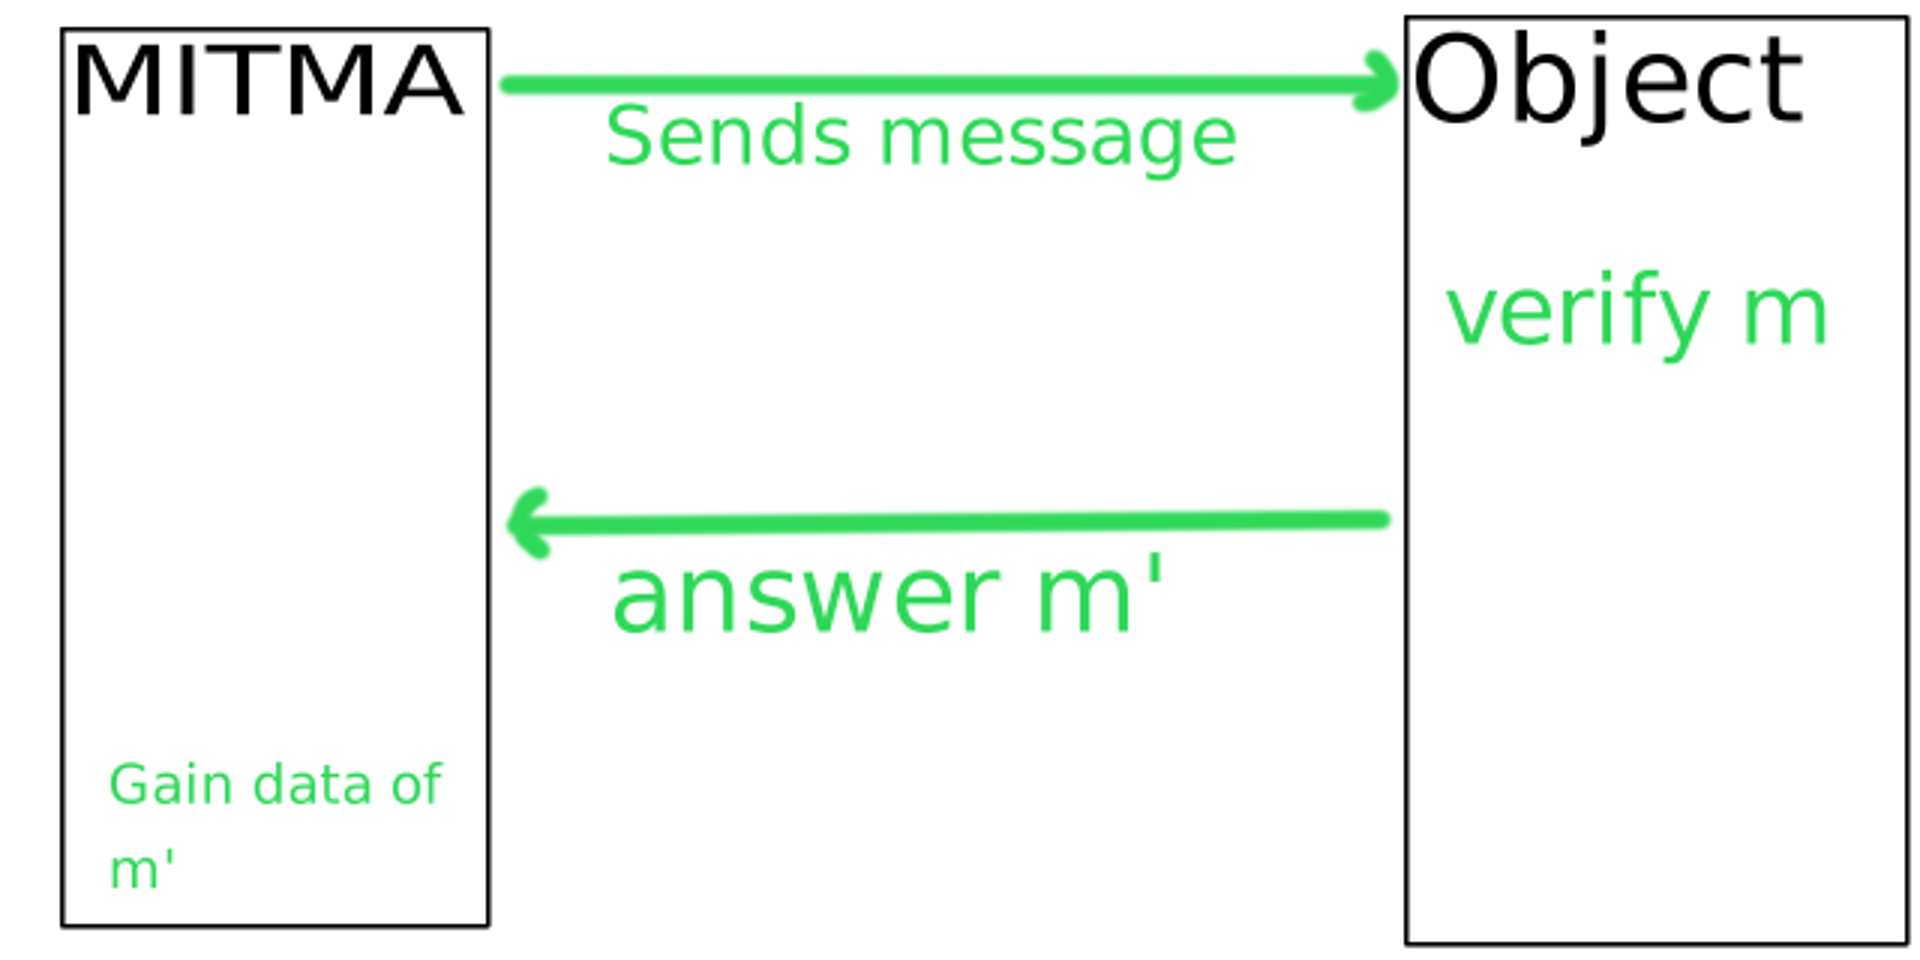
\includegraphics[width=3.3in,keepaspectratio]{./images/MITMA_send_received_msg.png}}

\usetikzlibrary{arrows}
\begin{tikzpicture}[->,>=stealth',shorten >=1pt,auto,node distance=1.3cm,
  thick,main node/.style={rectangle,fill=blue!5,draw,font=\sffamily\small}]

  \node[main node] (1) {
  						MITMA sends Message $m$
  					};
  \node[main node] (2) [below right of=1] {
  								 \Peer receives $m$
  								};
  \node[main node] (3) [below right of=2] {
  								 \Peer verifies $guard(m')$
  								};
  \node[main node] (4) [below left of=3] {
  								 \Peer if $guard(m')$ was valid, sends answer $m'$
  								};
  \node[main node] (5) [below left of=4] {
  								 MITMA gains knowledge of $m'$
  								};

  \path[every node/.style={font=\sffamily\small}]
    (1) edge node [] {} (2)
    (2) edge node [] {} (3)
    (3) edge node [] {} (4)
    (4) edge node [] {} (5)
    (5) edge [bend left=86] node [] {} (1)
        ;
\end{tikzpicture}
	
	\caption{Schematic of how an \MITMA gains knowledge}
	\label{fig:MITMAExample}
\end{figure}

\subsubsection{Message formula}

The \FOL formula for each sent message is constructed like this.
\linesep

Let $Messages(A) =_{def} \{ m_0 , ... , m_n \}$ be the set of all messages \Peer A receives or sends with 
\begin{small}
\begin{align*}
Receives(A) 		&=_{def} \{ m\ |\ m \in Messages(A) \wedge  				\\
				&\hspace{3em}  target(m) \not = A \wedge source(m) \not = A \}   \\
				& = \{ m_{r_0} , ... , m_{r_k} \}	\\
Sends(A)  		&=_{def} \{m\ |\ m \in Messages(A) \wedge  				\\
				&\hspace{3em}  source(m) \not = A \wedge target(m) \not = A \}   \\
				&= \{ m_{s_0} , ... , m_{s_j} \}	\\
m_{k} < m_{j} 	&=_{def} k < j 
\end{align*}
\end{small}

Then the constructed formula for each message $m \in Messages(A)$ is
%
\begin{small}
\begin{multline*}
	F_{m_{s_n}} = (
 		(\forall m_{r_q} \in Receives(A) . m_{s_{max(n-1,0)}} < m_{r_q} . \\ 
 		\hspace{4em} \forall i \in \mathbb{N}_0 . i \leq |args(m_{r_q})| : \knows{name(m_{r_q})_i}) \\
 		\wedge 
 		(guard(m))
 	)
 	\Rightarrow
	\forall a \in args(m_{s_n}) . \knows{a}
\end{multline*}
\end{small}

\subsection{Phase 2 : Check attackers knowledge}

In the second phase of the analysis, it is check whether or not a \MITMA 
knows specific values after successfully sniffing the whole communication.
\linesep

Let $seek = \{ val_0 , val_1 , ... val_n \}$ be a set of values, which are to be check whether a \MITMA is able 
to gain knowledge about them. If $\inknows{val_k} \Leftrightarrow val_k \text{ is compromised }$.

\subsection{Example Analysis}

\begin{figure}[!t]
	\centering
	\fbox{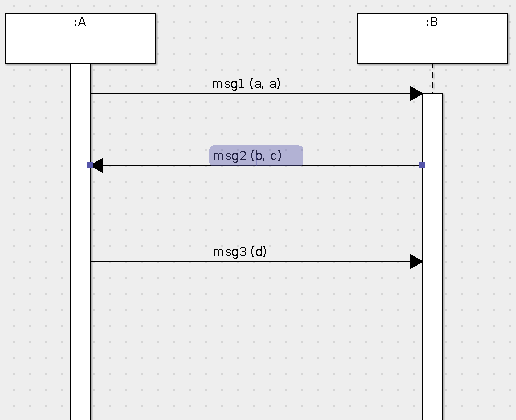
\includegraphics[width=3.3in,keepaspectratio]{./images/Example_UML_Diagram.png}}
	\caption{Example UML Sequence Diagram}
	\label{fig:ExampleAnalysisGraphic}
\end{figure}

Given the sequence diagram of figure~\ref{fig:ExampleAnalysisGraphic}, initial knowledge $knows = \emptyset$ and the following sets
\begin{small}
\begin{align*}
	Messages 	   =	& \{				
				  Msg1(a,a),		\\
				& Msg2(b,c),		\\
				& Msg3(d)		
				  \}				\\
	Messages(A) =	& \{				 
				  Msg1(a,a),		\\
				& Msg2(b,c),		\\
				& Msg3(d)		
				  \}				\\
	Messages(B) =	& \{				 
				  Msg1(a,a),		\\
				& Msg2(b,c),		\\
				& Msg3(d)		
				  \}				\\
  	Sends(A)	   =	& \{				 
				  Msg1(a,a),		\\
				& Msg3(d)		
				  \}				\\
  	Receives(A) =	& \{				 
				  Msg2(b,c)		
				  \}				\\
  	Sends(B)	   =	& \{				 
				  Msg2(b,c)		
				  \}				\\
  	Receives(B) =	& \{				 
				  Msg1(a,a),		\\
				& Msg3(d)		
				  \}				
\end{align*}
\begin{align*}
	Msg1(a,a) < Msg2(b,c) < Msg3(d) 
\end{align*}
\begin{align*}
	m_0			=& Msg1(a,a) 	\\
	m_1			=& Msg2(b,c) 	\\
	m_2 			=& Msg3(d)  	\\
	guard(m_0)	=& \text{[]}														\\
	guard(m_1)	=& \text{[ $Msg1_1$ = $Msg1_2$ ]}									\\
	guard(m_1)	=& \text{[ ($Msg2_1$ = b AND $Msg2_1$ = c) ]}							\\
	F_A 			=& F_{m_0} \implies F_{m_2} 										\\
	F_B 			=& F_{m_1} 														\\
	F_{m_0}		=& (\top \wedge guard(m_0)) \Rightarrow	\knows{a} \wedge \knows{a} 		\\
	F_{m_1}		=& ((\knows{Msg1_1} \wedge \knows{Msg1_2}) \wedge guard(m_1))			\\ 
			 	 & \Rightarrow	 \knows{b} \wedge \knows {c} 						\\
	F_{m_2}		=& ((\knows{Msg2_1} \wedge \knows{Msg2_2}) \wedge guard(m_2))  			\\
			 	 & \Rightarrow	\knows{d} 
\end{align*}
\begin{align*}
	KnowsFraction =& \{ 
	\knows{Msg1_1},
	\knows{Msg1_2}, \\
	& \knows{Msg2_1}, 
	\knows{Msg2_2}, \\
	& \knows{Msg3_1} 
	\}
	\\
	KnowsFraction \subset&\ \knowsname 
\end{align*}
\end{small}

A valid assignment would be e.g.
\begin{small}
\begin{align*}
	Msg1_1 = a \\
	Msg1_2 = a \\
	Msg2_1 = b \\
	Msg2_2 = c \\
	Msg3_1 = d 
\end{align*}
\end{small}

With this assignment $F_A$, $F_B$ are both true, which means communication 
isn't secure with \Peers A, B as a \MITMA is able to impersonate A and B.

\section{Analyzing using the CARiSMA Plugin}

% Grafik neu machen! 
\begin{figure}[!t]
	\centering
	\fbox{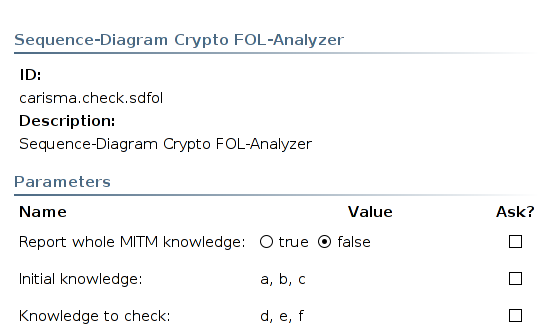
\includegraphics[width=3.3in,keepaspectratio]{./images/GUI_rightside.png}}
	\caption{\SDC Configuration}
	\label{fig:GUI}
\end{figure}

The usage of the plugin is quite easy. Firstly a valid UML Sequence Diagram 
in the .uml2 format is needed. \textbf{Papyrus} or \textbf{AlgoUML} may be use to create such 
an UML Sequence Diagram. Also the guards have to be valid under the syntax of ~\ref{subsubsec:guardssyntax}.
\linesep

Then load the .uml2 file in CARiSMA, select the \SDC, add initial knowledge (valid under the syntax of ~\ref{subsubsec:initialsyntax})
and knowledge which is to check whether or not the attacker is able to gain it (valid under the syntax of ~\ref{subsubsec:seeksyntax}).

% Grafik neu machen! 
\begin{figure}[!t]
	\centering
	\fbox{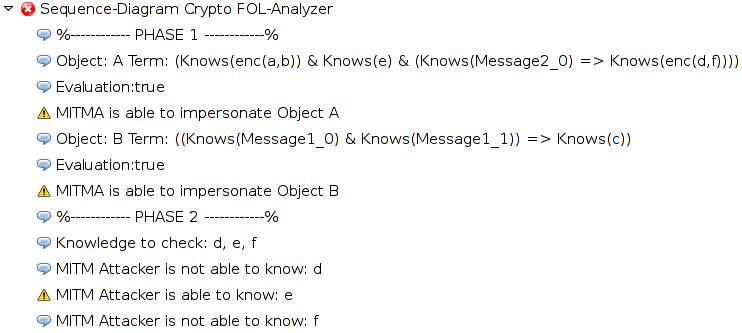
\includegraphics[width=3.3in,keepaspectratio]{./images/Example_Output.png}}
	\caption{Example Analysis Report}
	\label{fig:GUI}
\end{figure}

\section{References}

This Plugin is based on the work 
\textit{Werkzeugunterstützte Sicherheits-Analyse von kryptographischen Protokollen mit automatischen Theorem-Beweisern} 
(Tool supported security analysis of cryptographic protocols of automatic theorem solver) by \textbf{Andreas Gilg}.



%\subsection{Report whole Knowledge of \MITMA}

%As the Knowledge of the \MITMA is

%\subsection{Initial Knowledge}

%	\subsubsection{Syntax}

%\subsection{Knowledge to check}

%	\subsubsection{Syntax}
	
%\subsection{Example Analysis}

% Computer Society journal papers do something a tad strange with the very
% first section heading (almost always called "Introduction"). They place it
% ABOVE the main text! IEEEtran.cls currently does not do this for you.
% However, You can achieve this effect by making LaTeX jump through some
% hoops via something like:
%
%\ifCLASSOPTIONcompsoc
%  \noindent\raisebox{2\baselineskip}[0pt][0pt]%
%  {\parbox{\columnwidth}{\section{Introduction}\label{sec:introduction}%
%  \global\everypar=\everypar}}%
%  \vspace{-1\baselineskip}\vspace{-\parskip}\par
%\else
%  \section{Introduction}\label{sec:introduction}\par
%\fi
%
% Admittedly, this is a hack and may well be fragile, but seems to do the
% trick for me. Note the need to keep any \label that may be used right
% after \section in the above as the hack puts \section within a raised box.


%\hfill mds
 
%\hfill December 27, 2012

%\subsection{Subsection Heading Here}
%Subsection text here.

% needed in second column of first page if using \IEEEpubid
%\IEEEpubidadjcol

%\subsubsection{Subsubsection Heading Here}
%Subsubsection text here.


% An example of a floating figure using the graphicx package.
% Note that \label must occur AFTER (or within) \caption.
% For figures, \caption should occur after the \includegraphics.
% Note that IEEEtran v1.8 and later has special internal code that
% is designed to preserve the operation of \label within \caption
% even when the captionsoff option is in effect. However, because
% of issues like this, it may be the safest practice to put all your
% \label just after \caption rather than within \caption{}.
%
% Reminder: the "draftcls" or "draftclsnofoot", not "draft", class
% option should be used if it is desired that the figures are to be
% displayed while in draft mode.
%
%\begin{figure}[!t]
%\centering
%\includegraphics[width=2.5in]{myfigure}
% where an .eps filename suffix will be assumed under latex, 
% and a .pdf suffix will be assumed for pdflatex; or what has been declared
% via \DeclareGraphicsExtensions.
%\caption{Simulation Results.}
%\label{fig_sim}
%\end{figure}

% Note that IEEE typically puts floats only at the top, even when this
% results in a large percentage of a column being occupied by floats.
% However, the Computer Society has been known to put floats at the bottom.


% An example of a double column floating figure using two subfigures.
% (The subfig.sty package must be loaded for this to work.)
% The subfigure \label commands are set within each subfloat command,
% and the \label for the overall figure must come after \caption.
% \hfil is used as a separator to get equal spacing.
% Watch out that the combined width of all the subfigures on a 
% line do not exceed the text width or a line break will occur.
%
%\begin{figure*}[!t]
%\centering
%\subfloat[Case I]{\includegraphics[width=2.5in]{box}%
%\label{fig_first_case}}
%\hfil
%\subfloat[Case II]{\includegraphics[width=2.5in]{box}%
%\label{fig_second_case}}
%\caption{Simulation results.}
%\label{fig_sim}
%\end{figure*}
%
% Note that often IEEE papers with subfigures do not employ subfigure
% captions (using the optional argument to \subfloat[]), but instead will
% reference/describe all of them (a), (b), etc., within the main caption.


% An example of a floating table. Note that, for IEEE style tables, the 
% \caption command should come BEFORE the table. Table text will default to
% \footnotesize as IEEE normally uses this smaller font for tables.
% The \label must come after \caption as always.
%
%\begin{table}[!t]
%% increase table row spacing, adjust to taste
%\renewcommand{\arraystretch}{1.3}
% if using array.sty, it might be a good idea to tweak the value of
% \extrarowheight as needed to properly center the text within the cells
%\caption{An Example of a Table}
%\label{table_example}
%\centering
%% Some packages, such as MDW tools, offer better commands for making tables
%% than the plain LaTeX2e tabular which is used here.
%\begin{tabular}{|c||c|}
%\hline
%One & Two\\
%\hline
%Three & Four\\
%\hline
%\end{tabular}
%\end{table}


% Note that IEEE does not put floats in the very first column - or typically
% anywhere on the first page for that matter. Also, in-text middle ("here")
% positioning is not used. Most IEEE journals use top floats exclusively.
% However, Computer Society journals sometimes do use bottom floats - bear
% this in mind when choosing appropriate optional arguments for the
% figure/table environments.
% Note that, LaTeX2e, unlike IEEE journals, places footnotes above bottom
% floats. This can be corrected via the \fnbelowfloat command of the
% stfloats package.



%\section{Conclusion}
%The conclusion goes here.





% if have a single appendix:
%\appendix[Proof of the Zonklar Equations]
% or
%\appendix  % for no appendix heading
% do not use \section anymore after \appendix, only \section*
% is possibly needed

% use appendices with more than one appendix
% then use \section to start each appendix
% you must declare a \section before using any
% \subsection or using \label (\appendices by itself
% starts a section numbered zero.)
%


%\appendices
%\section{Proof of the First Zonklar Equation}
%Appendix one text goes here.
%
%% you can choose not to have a title for an appendix
%% if you want by leaving the argument blank
%\section{}
%Appendix two text goes here.
%
%
%% use section* for acknowledgement
%\ifCLASSOPTIONcompsoc
%  % The Computer Society usually uses the plural form
%  \section*{Acknowledgments}
%\else
%  % regular IEEE prefers the singular form
%  \section*{Acknowledgment}
%\fi
%
%
%The authors would like to thank...
%
%
%% Can use something like this to put references on a page
%% by themselves when using endfloat and the captionsoff option.
%\ifCLASSOPTIONcaptionsoff
%  \newpage
%\fi



% trigger a \newpage just before the given reference
% number - used to balance the columns on the last page
% adjust value as needed - may need to be readjusted if
% the document is modified later
%\IEEEtriggeratref{8}
% The "triggered" command can be changed if desired:
%\IEEEtriggercmd{\enlargethispage{-5in}}

% references section

% can use a bibliography generated by BibTeX as a .bbl file
% BibTeX documentation can be easily obtained at:
% http://www.ctan.org/tex-archive/biblio/bibtex/contrib/doc/
% The IEEEtran BibTeX style support page is at:
% http://www.michaelshell.org/tex/ieeetran/bibtex/
%\bibliographystyle{IEEEtran}
% argument is your BibTeX string definitions and bibliography database(s)
%\bibliography{IEEEabrv,../bib/paper}
%
% <OR> manually copy in the resultant .bbl file
% set second argument of \begin to the number of references
% (used to reserve space for the reference number labels box)
%\begin{thebibliography}{1}
%
%\bibitem{IEEEhowto:kopka}
%H.~Kopka and P.~W. Daly, \emph{A Guide to \LaTeX}, 3rd~ed.\hskip 1em plus
%  0.5em minus 0.4em\relax Harlow, England: Addison-Wesley, 1999.
%
%\end{thebibliography}

% biography section
% 
% If you have an EPS/PDF photo (graphicx package needed) extra braces are
% needed around the contents of the optional argument to biography to prevent
% the LaTeX parser from getting confused when it sees the complicated
% \includegraphics command within an optional argument. (You could create
% your own custom macro containing the \includegraphics command to make things
% simpler here.)
%\begin{IEEEbiography}[{\includegraphics[width=1in,height=1.25in,clip,keepaspectratio]{mshell}}]{Michael Shell}
% or if you just want to reserve a space for a photo:
%
%\begin{IEEEbiography}{Michael Shell}
%Biography text here.
%\end{IEEEbiography}
%
%% if you will not have a photo at all:
%\begin{IEEEbiographynophoto}{John Doe}
%Biography text here.
%\end{IEEEbiographynophoto}
%
%% insert where needed to balance the two columns on the last page with
%% biographies
%%\newpage
%
%\begin{IEEEbiographynophoto}{Jane Doe}
%Biography text here.
%\end{IEEEbiographynophoto}

% You can push biographies down or up by placing
% a \vfill before or after them. The appropriate
% use of \vfill depends on what kind of text is
% on the last page and whether or not the columns
% are being equalized.

%\vfill

% Can be used to pull up biographies so that the bottom of the last one
% is flush with the other column.
%\enlargethispage{-5in}



% that's all folks
\end{document}


